% supplement.tex - Supplementary material for snsm_rsl.tex. All tables are generated by
% experiments/make_paper_tables.py; never edit numbers by hand.
\documentclass[11pt]{article}
\usepackage[a4paper,margin=2cm]{geometry}
\usepackage{booktabs,graphicx,amsmath,amssymb,tikz}
\usetikzlibrary{positioning,arrows.meta}
\renewcommand{\thetable}{S\arabic{table}}
\renewcommand{\thefigure}{S\arabic{figure}}
\newcommand{\ntrainIP}{505}
\newcommand{\ntestIP}{9{,}744}
\newcommand{\ntrainKSC}{256}
\newcommand{\ntestKSC}{4{,}955}
\newcommand{\ntrainPU}{2{,}135}
\newcommand{\ntestPU}{40{,}641}
\newcommand{\ntrainBW}{156}
\newcommand{\ntestBW}{3{,}092}
\newcommand{\ntrainIPstd}{695}
\newcommand{\ntestIPstd}{9{,}671}
\newcommand{\ntrainIPcnt}{695}
\newcommand{\ntestIPcnt}{9{,}554}
\newcommand{\djtestPU}{33{,}847--36{,}453}
\newcommand{\djclassesPU}{9}
\newcommand{\djtestKSC}{3{,}077--3{,}513}
\newcommand{\djclassesKSC}{11}
\newcommand{\dropPU}{32.0}
\newcommand{\spreadDJPU}{1.80}
\newcommand{\dropKSC}{34.3}
\newcommand{\spreadDJKSC}{4.44}
\newcommand{\spreadIPRand}{3.84}
\newcommand{\spreadIPSmall}{0.60}
\newcommand{\spreadIPCnt}{0.14}
\newcommand{\spreadIPStd}{0.35}
\newcommand{\nsigIPrand}{5}
\newcommand{\ciwIPrand}{2.2}
\newcommand{\nsigIPcnt}{0}
\newcommand{\ciwIPcnt}{0.3}
\newcommand{\nsigIPstd}{1}
\newcommand{\ciwIPstd}{0.4}
\newcommand{\nsigPUdj}{0}
\newcommand{\ciwPUdj}{4.0}
\newcommand{\nsigKSCdj}{3}
\newcommand{\ciwKSCdj}{3.9}
\newcommand{\nsigIPsmall}{7}
\newcommand{\ciwIPsmall}{0.6}
\newcommand{\nsigPUscarce}{2}
\newcommand{\ciwPUscarce}{1.7}
\newcommand{\nsigKSCscarce}{0}
\newcommand{\ciwKSCscarce}{2.0}
\newcommand{\spreadSCIPfive}{3.84}
\newcommand{\spreadSCIPsmall}{0.60}
\newcommand{\spreadSCPUfive}{0.31}
\newcommand{\spreadSCPUscarce}{1.59}
\newcommand{\spreadSCKSCfive}{0.32}
\newcommand{\spreadSCKSCscarce}{1.65}
\newcommand{\ipRandGain}{1.75--3.84}
\newcommand{\ipRandGainShort}{1.8--3.8}
\newcommand{\ipRandGainInt}{2--4}
\newcommand{\randOtherSpread}{0.32}
\newcommand{\kscFixedRange}{99.2--99.5}
\newcommand{\pcGpmDisp}{80.0--84.4}
\newcommand{\pcGpmRest}{62.7--78.5}
\newcommand{\pcOatsDisp}{66.3--77.2}
\newcommand{\pcOatsRest}{36.8--56.1}
\newcommand{\pcAlfalfaSpread}{3.3}
\newcommand{\cntCImax}{0.3}
\newcommand{\stdEcaDiff}{0.33}
\newcommand{\smallGain}{0.30--0.60}
\newcommand{\spreadSCIPsmallShort}{0.6}
\newcommand{\dropScarcePU}{15}
\newcommand{\dropScarceKSC}{7}
\newcommand{\djOAPU}{55--57}
\newcommand{\djOAKSC}{74--77}
\newcommand{\dropRange}{32--34}
\newcommand{\djStdRange}{4.4--7.4}
\newcommand{\ablMeanDrop}{1.16}
\newcommand{\paramsEca}{6}
\newcommand{\paramsSe}{4{,}256}
\newcommand{\paramsSnsm}{260}
\newcommand{\latencyRatio}{3.7}
\newcommand{\trainRatio}{1.7}
\newcommand{\margin}{1}
\newcommand{\seedSdIP}{2.2}
\newcommand{\bhSig}{16}
\newcommand{\bhTotal}{56}
\newcommand{\holmSig}{18}
\newcommand{\nSettings}{8}
\newcommand{\neqPUscarce}{1}
\newcommand{\neqKSCscarce}{2}
\newcommand{\ipRandOAspread}{0.17}
\newcommand{\nseedsIP}{15}


\begin{document}
\begin{center}
{\large\bfseries Supplementary material}\\[4pt]
Channel attention in lightweight hyperspectral CNNs: an equivalence-tested comparison
\end{center}

\begin{figure}[h]
\centering
\resizebox{0.85\textwidth}{!}{% SNSM modulation inside a residual block (TikZ; included from snsm_rsl.tex).
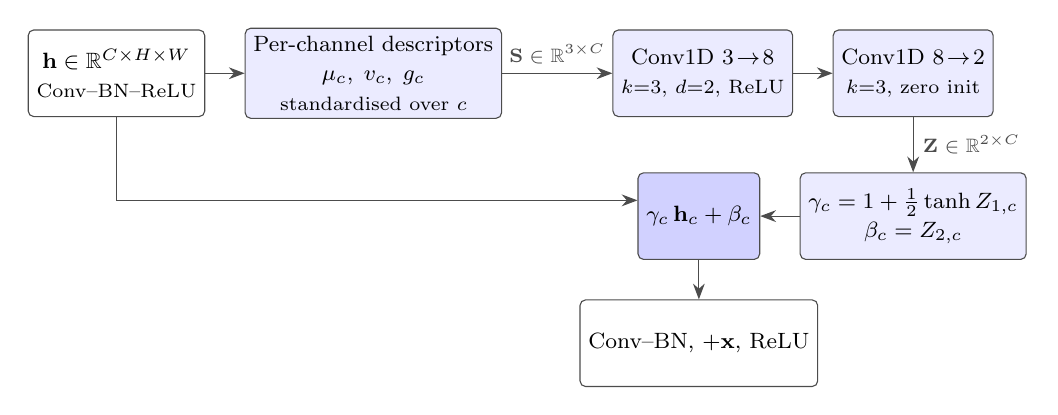
\begin{tikzpicture}[
  font=\footnotesize, node distance=4mm and 5mm,
  box/.style={draw=black!70, rounded corners=2pt, align=center, minimum height=11mm, inner sep=3pt},
  op/.style={box, fill=blue!8},
  arr/.style={-{Stealth[length=2mm]}, black!70}]
\node[box] (h) {$\mathbf{h}\in\mathbb{R}^{C\times H\times W}$\\[1pt]\scriptsize Conv--BN--ReLU};
\node[op, right=of h] (d) {Per-channel descriptors\\[1pt]$\mu_c,\; v_c,\; g_c$\\[1pt]\scriptsize standardised over $c$};
\node[op, right=14mm of d] (c1) {Conv1D $3\!\to\!8$\\[1pt]\scriptsize $k{=}3$, $d{=}2$, ReLU};
\node[op, right=of c1] (c2) {Conv1D $8\!\to\!2$\\[1pt]\scriptsize $k{=}3$, zero init};
\node[op, below=7mm of c2] (gb) {$\gamma_c=1+\tfrac12\tanh Z_{1,c}$\\[1pt]$\beta_c=Z_{2,c}$};
\node[box, left=of gb, fill=blue!18] (m) {$\gamma_c\,\mathbf{h}_c+\beta_c$};
\node[box, below=5mm of m] (out) {Conv--BN, $+\mathbf{x}$, ReLU};
\draw[arr] (h) -- (d);
\draw[arr] (d) -- node[above]{\scriptsize $\mathbf{S}\in\mathbb{R}^{3\times C}$} (c1);
\draw[arr] (c1) -- (c2);
\draw[arr] (c2) -- node[right]{\scriptsize $\mathbf{Z}\in\mathbb{R}^{2\times C}$} (gb);
\draw[arr] (gb) -- (m);
\draw[arr] (h.south) |- ([yshift=2mm]m.west) ;
\draw[arr] (m) -- (out);
\end{tikzpicture}
}
\caption{The SNSM probe inside a residual block. Per-channel descriptors of the feature map $\mathbf{h}$ (mean, variance, cross-channel gradient) are filtered along the channel axis by two one-dimensional convolutions, whose output sets a bounded scale $\gamma_c$ and a shift $\beta_c$ for each channel. The second convolution starts at zero, so the block is initially the identity.}
\end{figure}

\begin{table}[h]
\centering
\caption{Random 5\% splits: OA and AA (\%, mean $\pm$ std) of all models, including an FC ($\gamma{+}\beta$) gate and two external baselines trained under the same protocol, HybridSN (original layer configuration) and SSFTT (four tokens, one transformer layer with eight heads). The eight backbone variants use 15 seeds on IP and five elsewhere; the other models use five.}
\resizebox{\textwidth}{!}{\begin{tabular}{lcccccccc}
\toprule
Method & \multicolumn{2}{c}{IP} & \multicolumn{2}{c}{KSC} & \multicolumn{2}{c}{PU} & \multicolumn{2}{c}{BW} \\
 & OA & AA & OA & AA & OA & AA & OA & AA \\
\midrule
Plain CNN & 96.28$\pm$0.79 & 89.49$\pm$2.44 & 99.65$\pm$0.34 & 99.51$\pm$0.36 & \textbf{99.59$\pm$0.07} & 99.01$\pm$0.16 & 99.09$\pm$0.55 & 98.87$\pm$0.90 \\
SE ($\gamma$) & 96.34$\pm$0.62 & 90.04$\pm$2.18 & 99.61$\pm$0.28 & 99.43$\pm$0.38 & 99.53$\pm$0.19 & 98.80$\pm$0.56 & 98.95$\pm$0.82 & 98.76$\pm$1.07 \\
ECA ($\gamma$) & 96.28$\pm$0.68 & 90.87$\pm$2.53 & 99.61$\pm$0.47 & 99.40$\pm$0.66 & 99.58$\pm$0.10 & 99.00$\pm$0.20 & \textbf{99.13$\pm$0.76} & \textbf{98.90$\pm$1.08} \\
CBAM & 96.19$\pm$0.60 & 91.58$\pm$1.49 & 99.54$\pm$0.56 & 99.23$\pm$0.83 & 99.58$\pm$0.06 & \textbf{99.11$\pm$0.18} & 98.99$\pm$0.87 & 98.78$\pm$1.20 \\
GCT & 96.28$\pm$0.80 & 90.07$\pm$2.34 & \textbf{99.69$\pm$0.26} & \textbf{99.55$\pm$0.28} & 99.58$\pm$0.08 & 98.99$\pm$0.18 & 99.11$\pm$0.56 & 98.88$\pm$0.91 \\
SRM & 96.20$\pm$0.71 & 93.04$\pm$2.14 & 99.69$\pm$0.36 & 99.51$\pm$0.49 & 99.55$\pm$0.07 & 98.92$\pm$0.17 & 98.87$\pm$0.63 & 98.67$\pm$0.97 \\
SNSM ($\gamma$) & 96.17$\pm$0.73 & 92.89$\pm$2.00 & 99.69$\pm$0.26 & 99.50$\pm$0.39 & 99.49$\pm$0.05 & 98.91$\pm$0.16 & 99.10$\pm$0.62 & 98.89$\pm$0.96 \\
SNSM ($\gamma{+}\beta$) & 96.27$\pm$0.67 & \textbf{93.33$\pm$1.68} & 99.63$\pm$0.55 & 99.45$\pm$0.73 & 99.47$\pm$0.05 & 98.93$\pm$0.16 & 99.04$\pm$0.69 & 98.85$\pm$1.03 \\
\midrule
FC ($\gamma{+}\beta$) & 96.24$\pm$0.52 & 92.51$\pm$1.60 & 99.63$\pm$0.40 & 99.48$\pm$0.47 & 99.51$\pm$0.06 & 98.88$\pm$0.14 & 98.80$\pm$0.70 & 98.63$\pm$0.98 \\
HybridSN & 88.30$\pm$4.91 & 73.64$\pm$8.28 & 95.00$\pm$3.02 & 91.20$\pm$5.32 & 97.84$\pm$1.52 & 95.46$\pm$4.12 & 77.16$\pm$37.92 & 75.56$\pm$38.31 \\
SSFTT & \textbf{96.71$\pm$0.79} & 92.35$\pm$1.81 & 99.38$\pm$0.28 & 99.15$\pm$0.32 & -- & -- & -- & -- \\
\bottomrule
\end{tabular}
}
\end{table}

\begin{table}[h]
\centering
\caption{Paired AA differences SNSM ($\gamma{+}\beta$) $-$ block (points) with 95\% $t$ intervals, for every setting of the main paper's paired table.}
\resizebox{\textwidth}{!}{\begin{tabular}{lcccccccc}
\toprule
Setting & Plain & SE & ECA & CBAM & GCT & SRM & SNSM ($\gamma$) & Seeds \\
\midrule
IP, random 5\% & +3.84 [+2.4, +5.3] & +3.29 [+2.2, +4.4] & +2.45 [+0.9, +4.0] & +1.75 [+0.9, +2.6] & +3.26 [+2.0, +4.6] & +0.29 [-0.8, +1.4] & +0.44 [-0.3, +1.2] & 15 \\
IP, smallest 15 & +0.39 [+0.1, +0.7] & +0.50 [+0.3, +0.7] & +0.33 [+0.1, +0.6] & +0.60 [+0.3, +0.9] & +0.35 [+0.0, +0.7] & +0.41 [+0.0, +0.8] & +0.30 [+0.1, +0.5] & 15 \\
IP, random 50/15 & -0.01 [-0.2, +0.2] & -0.08 [-0.2, +0.1] & +0.04 [-0.1, +0.2] & +0.05 [-0.1, +0.2] & +0.01 [-0.2, +0.2] & +0.07 [-0.1, +0.2] & +0.06 [-0.2, +0.3] & 15 \\
IP, standard & +0.24 [+0.0, +0.4] & +0.23 [+0.0, +0.4] & +0.33 [+0.2, +0.5] & +0.04 [-0.2, +0.2] & +0.25 [+0.1, +0.4] & -0.02 [-0.2, +0.2] & +0.12 [-0.1, +0.3] & 15 \\
\midrule
PU, smallest 1/1/2 & -0.59 [-1.6, +0.4] & -0.74 [-1.6, +0.1] & -1.19 [-1.9, -0.5] & -0.30 [-1.1, +0.5] & -1.14 [-2.2, -0.1] & -0.55 [-1.2, +0.2] & -1.59 [-2.6, -0.5] & 15 \\
KSC, smallest 1/1/2 & -0.24 [-0.9, +0.5] & +0.79 [+0.1, +1.4] & +0.39 [-0.6, +1.4] & +0.54 [-0.7, +1.8] & -0.21 [-1.0, +0.5] & +1.41 [+0.3, +2.5] & +0.03 [-1.3, +1.3] & 15 \\
PU, hardest 1/1/2 & +0.97 [-0.1, +2.1] & +0.98 [-0.2, +2.1] & +0.64 [-0.5, +1.8] & +0.96 [-0.4, +2.3] & +0.77 [-0.2, +1.8] & +0.79 [-0.3, +1.9] & -0.82 [-1.5, -0.1] & 15 \\
KSC, hardest 1/1/2 & +0.71 [-0.0, +1.4] & +0.88 [-0.1, +1.8] & +0.20 [-0.5, +0.9] & +1.14 [+0.3, +2.0] & +0.77 [+0.1, +1.4] & +0.66 [-0.3, +1.6] & +0.90 [-0.3, +2.1] & 15 \\
\midrule
WHU, random 5\% & -0.06 [-0.1, +0.0] & -0.01 [-0.1, +0.1] & -0.02 [-0.1, +0.0] & +0.00 [-0.1, +0.1] & +0.00 [-0.1, +0.1] & -0.06 [-0.2, +0.0] & -0.03 [-0.1, +0.1] & 10 \\
PU, patch-disjoint & +0.31 [-1.9, +2.5] & -0.47 [-2.7, +1.8] & -0.39 [-2.4, +1.7] & +1.03 [-0.7, +2.8] & +0.92 [-1.0, +2.8] & +1.33 [-0.4, +3.1] & +0.03 [-2.0, +2.0] & 15 \\
KSC, patch-disjoint & +3.46 [+1.5, +5.4] & -0.19 [-2.3, +1.9] & +1.86 [+0.3, +3.4] & +0.91 [-0.9, +2.7] & +3.51 [+1.5, +5.5] & +4.25 [+1.7, +6.8] & +1.40 [-1.0, +3.8] & 15 \\
WHU, patch-disjoint & -2.01 [-3.3, -0.7] & -2.39 [-4.8, +0.1] & -1.77 [-4.5, +1.0] & -1.85 [-3.6, -0.1] & -1.32 [-3.3, +0.6] & -0.84 [-2.7, +1.0] & -0.46 [-3.0, +2.1] & 10 \\
\midrule
IP, random 5\%, deeper host & -0.53 [-1.4, +0.3] & +0.14 [-0.6, +0.9] & +0.18 [-0.5, +0.9] & -0.35 [-1.2, +0.5] & -0.51 [-1.3, +0.2] & -0.87 [-2.2, +0.5] & -0.19 [-1.3, +0.9] & 10 \\
KSC, patch-disjoint, deeper host & -1.88 [-4.9, +1.1] & -0.80 [-5.5, +3.9] & -2.87 [-5.2, -0.6] & -1.35 [-4.7, +2.0] & -1.63 [-4.6, +1.3] & +0.34 [-2.8, +3.4] & -2.00 [-5.6, +1.6] & 10 \\
KSC, patch-disjoint, train-only PCA & +0.33 [-2.3, +2.9] & -0.98 [-3.1, +1.2] & -0.01 [-2.4, +2.4] & -2.38 [-4.1, -0.7] & +0.54 [-2.0, +3.1] & +1.65 [-0.7, +4.0] & -0.38 [-2.8, +2.1] & 15 \\
IP, random 5\%, lr $3\times10^{-4}$ & +8.16 [+6.8, +9.5] & +7.42 [+4.8, +10.0] & +8.26 [+5.4, +11.2] & +6.12 [+3.5, +8.8] & +8.06 [+6.7, +9.4] & +5.37 [+4.1, +6.6] & +5.27 [+3.1, +7.4] & 5 \\
IP, random 5\%, lr $3\times10^{-3}$ & +0.98 [-0.0, +2.0] & +1.48 [+0.2, +2.8] & +0.56 [-0.3, +1.4] & +0.80 [-0.3, +1.9] & +0.83 [+0.0, +1.7] & +0.28 [-0.8, +1.3] & -0.03 [-1.2, +1.2] & 15 \\
\bottomrule
\end{tabular}
}
\end{table}

\begin{table}[h]
\centering
\caption{Paired AA differences block $-$ plain CNN (points), so that no block is the reference. $^{*}$: Holm-corrected Wilcoxon $p<0.05$ within the row (seven comparisons); $^{\dagger}$: equivalent within $\pm$\margin\ point (paired TOST). GCT stays close to the plain CNN in most settings because its gate starts at the identity.}
\resizebox{\textwidth}{!}{\begin{tabular}{lccccccc}
\toprule
Setting & SE & ECA & CBAM & GCT & SRM & SNSM ($\gamma$) & SNSM ($\gamma{+}\beta$) \\
\midrule
IP, random 5\% & +0.55 & +1.38 & +2.09$^{*}$ & +0.58$^{*}$$^{\dagger}$ & +3.55$^{*}$ & +3.40$^{*}$ & +3.84$^{*}$ \\
IP, smallest 15 & -0.11$^{\dagger}$ & +0.06$^{\dagger}$ & -0.20$^{\dagger}$ & +0.04$^{\dagger}$ & -0.02$^{\dagger}$ & +0.09$^{\dagger}$ & +0.39$^{*}$$^{\dagger}$ \\
IP, random 50/15 & +0.07$^{\dagger}$ & -0.05$^{\dagger}$ & -0.06$^{\dagger}$ & -0.01$^{\dagger}$ & -0.08$^{\dagger}$ & -0.07$^{\dagger}$ & -0.01$^{\dagger}$ \\
IP, standard & +0.01$^{\dagger}$ & -0.09$^{\dagger}$ & +0.21$^{\dagger}$ & -0.01$^{\dagger}$ & +0.26$^{*}$$^{\dagger}$ & +0.13$^{\dagger}$ & +0.24$^{\dagger}$ \\
\midrule
PU, smallest 1/1/2 & +0.15$^{\dagger}$ & +0.60 & -0.29 & +0.55$^{\dagger}$ & -0.05$^{\dagger}$ & +0.99 & -0.59 \\
KSC, smallest 1/1/2 & -1.03$^{*}$ & -0.63 & -0.78 & -0.03$^{\dagger}$ & -1.65$^{*}$ & -0.27 & -0.24$^{\dagger}$ \\
PU, hardest 1/1/2 & -0.01$^{\dagger}$ & +0.33 & +0.01$^{\dagger}$ & +0.20$^{\dagger}$ & +0.18$^{\dagger}$ & +1.79$^{*}$ & +0.97 \\
KSC, hardest 1/1/2 & -0.17$^{\dagger}$ & +0.52 & -0.43 & -0.06$^{\dagger}$ & +0.06$^{\dagger}$ & -0.19 & +0.71 \\
\midrule
WHU, random 5\% & -0.05$^{\dagger}$ & -0.03$^{\dagger}$ & -0.06$^{\dagger}$ & -0.06$^{\dagger}$ & +0.00$^{\dagger}$ & -0.03$^{\dagger}$ & -0.06$^{\dagger}$ \\
PU, patch-disjoint & +0.78 & +0.70 & -0.72 & -0.61 & -1.02 & +0.28 & +0.31 \\
KSC, patch-disjoint & +3.65$^{*}$ & +1.60 & +2.55 & -0.06$^{\dagger}$ & -0.79 & +2.06 & +3.46$^{*}$ \\
WHU, patch-disjoint & +0.37 & -0.24 & -0.16 & -0.69 & -1.17 & -1.55 & -2.01 \\
PU, block-disjoint & -1.53 & -0.82 & -4.49$^{*}$ & +0.27$^{\dagger}$ & -2.63$^{*}$ & -2.61$^{*}$ & -3.77$^{*}$ \\
KSC, block-disjoint & +1.04 & +0.36 & -0.07 & -0.06$^{\dagger}$ & -2.27 & +0.61 & -0.63 \\
\midrule
IP, random 5\%, deeper host & -0.67 & -0.70 & -0.18$^{\dagger}$ & -0.01$^{\dagger}$ & +0.34 & -0.33 & -0.53 \\
KSC, patch-disjoint, deeper host & -1.08 & +0.98 & -0.54 & -0.25 & -2.22 & +0.12 & -1.88 \\
KSC, patch-disjoint, train-only PCA & +1.31 & +0.35 & +2.71 & -0.20$^{\dagger}$ & -1.32 & +0.72 & +0.33 \\
IP, random 5\%, lr $3\times10^{-4}$ & +0.74 & -0.10 & +2.04 & +0.10$^{\dagger}$ & +2.79 & +2.89 & +8.16 \\
IP, random 5\%, lr $3\times10^{-3}$ & -0.50 & +0.42 & +0.18 & +0.14$^{\dagger}$ & +0.70 & +1.01 & +0.98 \\
\bottomrule
\end{tabular}
}
\end{table}

\begin{table}[h]
\centering
\caption{Sensitivity to the equivalence margin: number of the seven comparisons SNSM ($\gamma{+}\beta$) $-$ block per setting that are equivalent (paired TOST, $\alpha=0.05$) within $\pm$0.5, $\pm$1 (main paper) and $\pm$2 AA points.}
\begin{tabular}{lccc}
\toprule
Setting & $\pm$0.5 & $\pm$1 & $\pm$2 \\
\midrule
IP, random 5\% & 0 & 0 & 2 \\
IP, smallest 15 & 1 & 7 & 7 \\
IP, random 50/15 & 7 & 7 & 7 \\
IP, standard & 7 & 7 & 7 \\
\midrule
PU, smallest 1/1/2 & 0 & 1 & 5 \\
KSC, smallest 1/1/2 & 0 & 2 & 6 \\
PU, hardest 1/1/2 & 0 & 0 & 6 \\
KSC, hardest 1/1/2 & 0 & 1 & 7 \\
\midrule
WHU, random 5\% & 7 & 7 & 7 \\
PU, patch-disjoint & 0 & 0 & 1 \\
KSC, patch-disjoint & 0 & 0 & 1 \\
WHU, patch-disjoint & 0 & 0 & 0 \\
\midrule
IP, random 5\%, deeper host & 0 & 2 & 7 \\
KSC, patch-disjoint, deeper host & 0 & 0 & 0 \\
KSC, patch-disjoint, train-only PCA & 0 & 0 & 1 \\
IP, random 5\%, lr $3\times10^{-4}$ & 0 & 0 & 0 \\
IP, random 5\%, lr $3\times10^{-3}$ & 0 & 0 & 6 \\
\bottomrule
\end{tabular}

\end{table}

\begin{table}[h]
\centering
\caption{Paired OA differences SNSM ($\gamma{+}\beta$) $-$ block (points). $^{*}$: Holm-corrected Wilcoxon $p<0.05$ within the row; $^{\dagger}$: equivalent within $\pm$\margin\ point (paired TOST).}
\resizebox{\textwidth}{!}{\begin{tabular}{lcccccccc}
\toprule
Setting & Plain & SE & ECA & CBAM & GCT & SRM & SNSM ($\gamma$) & Seeds \\
\midrule
IP, random 5\% & -0.01$^{\dagger}$ & -0.06$^{\dagger}$ & -0.01$^{\dagger}$ & +0.08$^{\dagger}$ & -0.00$^{\dagger}$ & +0.07$^{\dagger}$ & +0.11$^{\dagger}$ & 15 \\
IP, smallest 15 & -0.14$^{\dagger}$ & -0.12$^{\dagger}$ & -0.11$^{\dagger}$ & +0.04$^{\dagger}$ & -0.12$^{\dagger}$ & +0.02$^{\dagger}$ & +0.09$^{\dagger}$ & 15 \\
IP, random 50/15 & +0.04$^{\dagger}$ & -0.15$^{\dagger}$ & +0.09$^{\dagger}$ & +0.12$^{\dagger}$ & +0.06$^{\dagger}$ & +0.10$^{\dagger}$ & +0.01$^{\dagger}$ & 15 \\
IP, standard & +0.08$^{\dagger}$ & +0.34$^{\dagger}$ & +0.31$^{\dagger}$ & +0.14$^{\dagger}$ & +0.15$^{\dagger}$ & +0.03$^{\dagger}$ & +0.16$^{\dagger}$ & 15 \\
\midrule
PU, smallest 1/1/2 & -0.25$^{\dagger}$ & -0.26$^{\dagger}$ & -0.39$^{*}$$^{\dagger}$ & -0.10$^{\dagger}$ & -0.39$^{\dagger}$ & -0.18$^{\dagger}$ & -0.47$^{*}$$^{\dagger}$ & 15 \\
KSC, smallest 1/1/2 & -0.20$^{\dagger}$ & +0.23$^{\dagger}$ & +0.17$^{\dagger}$ & +0.19$^{\dagger}$ & -0.19$^{\dagger}$ & +0.50$^{\dagger}$ & -0.03$^{\dagger}$ & 15 \\
PU, hardest 1/1/2 & +0.53 & +0.58 & +0.31$^{\dagger}$ & +0.50 & +0.40$^{\dagger}$ & +0.50 & -0.55$^{\dagger}$ & 15 \\
KSC, hardest 1/1/2 & +0.75 & +0.68$^{*}$ & +0.29$^{\dagger}$ & +0.95$^{*}$ & +0.80 & +0.56 & +0.43 & 15 \\
\midrule
WHU, random 5\% & -0.04$^{\dagger}$ & -0.01$^{\dagger}$ & -0.01$^{\dagger}$ & -0.02$^{\dagger}$ & -0.03$^{\dagger}$ & -0.05$^{\dagger}$ & -0.02$^{\dagger}$ & 10 \\
PU, patch-disjoint & +1.50 & +0.89 & +0.51 & +0.69 & +2.21 & +0.79 & +1.39 & 15 \\
KSC, patch-disjoint & +1.98 & +0.32 & +0.72 & +0.43 & +1.91 & +2.75 & +0.25 & 15 \\
WHU, patch-disjoint & -2.51 & -2.86 & -1.22 & -1.22 & -0.24 & -2.61 & +0.07 & 10 \\
\midrule
IP, random 5\%, deeper host & -0.41$^{\dagger}$ & -0.26$^{\dagger}$ & -0.26$^{\dagger}$ & -0.34$^{\dagger}$ & -0.39$^{\dagger}$ & -0.27$^{\dagger}$ & -0.18$^{\dagger}$ & 10 \\
KSC, patch-disjoint, deeper host & -1.12 & -0.79 & -2.40 & -1.66 & -1.23 & +1.66 & -2.13 & 10 \\
KSC, patch-disjoint, train-only PCA & -0.74 & -0.65 & +0.23 & -2.17 & -0.67 & -0.22 & -0.78 & 15 \\
IP, random 5\%, lr $3\times10^{-4}$ & +0.45$^{\dagger}$ & +0.29$^{\dagger}$ & +0.29$^{\dagger}$ & -0.06$^{\dagger}$ & +0.46$^{\dagger}$ & +0.27$^{\dagger}$ & +0.18$^{\dagger}$ & 5 \\
IP, random 5\%, lr $3\times10^{-3}$ & -0.23$^{\dagger}$ & -0.03$^{\dagger}$ & -0.23$^{\dagger}$ & -0.26$^{\dagger}$ & -0.22$^{\dagger}$ & -0.12$^{\dagger}$ & -0.07$^{\dagger}$ & 15 \\
\bottomrule
\end{tabular}
}
\end{table}

\begin{table}[h]
\centering
\caption{AA (\%, mean $\pm$ std) of random 5\% splits and of the same splits with only the three smallest classes changed (15 seeds; the unchanged PU and KSC splits use five). The last row is the range of the block means.}
\resizebox{\textwidth}{!}{\begin{tabular}{lcccccc}
\toprule
Block & IP, 5\% & IP, smallest 15 & PU, 5\% & PU, smallest 1/1/2 & KSC, 5\% & KSC, smallest 1/1/2 \\
\midrule
Plain CNN & 89.49$\pm$2.44 & 96.03$\pm$0.76 & 99.01$\pm$0.16 & 84.20$\pm$3.43 & 99.51$\pm$0.36 & \textbf{93.12$\pm$3.44} \\
SE & 90.04$\pm$2.18 & 95.93$\pm$0.64 & 98.80$\pm$0.56 & 84.35$\pm$3.29 & 99.43$\pm$0.38 & 92.09$\pm$3.25 \\
ECA & 90.87$\pm$2.53 & 96.10$\pm$0.76 & 99.00$\pm$0.20 & 84.80$\pm$3.23 & 99.40$\pm$0.66 & 92.48$\pm$3.19 \\
CBAM & 91.58$\pm$1.49 & 95.83$\pm$0.67 & \textbf{99.11$\pm$0.18} & 83.91$\pm$2.11 & 99.23$\pm$0.83 & 92.34$\pm$4.15 \\
GCT & 90.07$\pm$2.34 & 96.07$\pm$0.75 & 98.99$\pm$0.18 & 84.74$\pm$3.75 & \textbf{99.55$\pm$0.28} & 93.09$\pm$3.24 \\
SRM & 93.04$\pm$2.14 & 96.01$\pm$0.81 & 98.92$\pm$0.17 & 84.15$\pm$3.45 & 99.51$\pm$0.49 & 91.47$\pm$3.62 \\
SNSM ($\gamma$) & 92.89$\pm$2.00 & 96.13$\pm$0.72 & 98.91$\pm$0.16 & \textbf{85.19$\pm$3.48} & 99.50$\pm$0.39 & 92.84$\pm$3.64 \\
SNSM ($\gamma{+}\beta$) & \textbf{93.33$\pm$1.68} & \textbf{96.43$\pm$0.66} & 98.93$\pm$0.16 & 83.60$\pm$2.96 & 99.45$\pm$0.73 & 92.88$\pm$3.12 \\
\midrule
Range of block means & 3.84 & 0.60 & 0.31 & 1.59 & 0.32 & 1.65 \\
\bottomrule
\end{tabular}
}
\end{table}

\begin{table}[h]
\centering
\caption{Robustness checks: AA (\%, mean $\pm$ std) of the eight backbone variants on block-disjoint splits of PU and KSC (15 seeds), in a deeper, wider host (four residual blocks of 128 channels; ten seeds), with PCA fitted on training pixels only (15 seeds), with the three hardest classes reduced to 1, 1 and 2 training pixels (15 seeds), and with learning rates $3\times10^{-4}$ (five seeds) and $3\times10^{-3}$ (15 seeds). The last row is the range of the block means.}
\resizebox{\textwidth}{!}{\begin{tabular}{lccccccccc}
\toprule
Block & PU, block-disj. & KSC, block-disj. & IP, deeper & KSC disj., deeper & KSC disj., train PCA & PU, hardest & KSC, hardest & IP, lr 3e-4 & IP, lr 3e-3 \\
\midrule
Plain CNN & 83.20$\pm$4.34 & 71.45$\pm$6.96 & 93.85$\pm$1.69 & 60.46$\pm$5.77 & 64.26$\pm$4.88 & 73.19$\pm$2.03 & 88.17$\pm$1.35 & 80.23$\pm$1.51 & 92.15$\pm$2.12 \\
SE & 81.67$\pm$4.89 & \textbf{72.48$\pm$7.42} & 93.18$\pm$2.02 & 59.38$\pm$6.05 & 65.57$\pm$5.03 & 73.17$\pm$2.09 & 88.01$\pm$1.39 & 80.97$\pm$1.99 & 91.65$\pm$1.84 \\
ECA & 82.38$\pm$4.21 & 71.81$\pm$8.11 & 93.14$\pm$1.80 & \textbf{61.44$\pm$6.66} & 64.61$\pm$4.56 & 73.52$\pm$2.28 & 88.69$\pm$1.92 & 80.13$\pm$2.35 & 92.57$\pm$1.93 \\
CBAM & 78.71$\pm$4.62 & 71.38$\pm$6.95 & 93.67$\pm$1.95 & 59.92$\pm$6.28 & \textbf{66.97$\pm$6.19} & 73.20$\pm$2.22 & 87.74$\pm$2.14 & 82.27$\pm$1.98 & 92.33$\pm$1.75 \\
GCT & \textbf{83.46$\pm$4.31} & 71.38$\pm$6.93 & 93.83$\pm$1.61 & 60.21$\pm$6.45 & 64.06$\pm$5.14 & 73.39$\pm$2.05 & 88.11$\pm$1.45 & 80.33$\pm$1.43 & 92.30$\pm$2.04 \\
SRM & 80.57$\pm$4.08 & 69.18$\pm$7.01 & \textbf{94.19$\pm$1.91} & 58.24$\pm$5.28 & 62.94$\pm$5.31 & 73.37$\pm$2.56 & 88.23$\pm$2.26 & 83.02$\pm$1.64 & 92.85$\pm$1.75 \\
SNSM ($\gamma$) & 80.59$\pm$4.79 & 72.06$\pm$6.56 & 93.51$\pm$1.59 & 60.58$\pm$5.41 & 64.98$\pm$7.02 & \textbf{74.98$\pm$2.65} & 87.98$\pm$2.44 & 83.12$\pm$1.49 & \textbf{93.16$\pm$1.89} \\
SNSM ($\gamma{+}\beta$) & 79.43$\pm$5.06 & 70.82$\pm$7.87 & 93.32$\pm$2.21 & 58.58$\pm$7.23 & 64.59$\pm$6.63 & 74.16$\pm$2.58 & \textbf{88.89$\pm$1.34} & \textbf{88.39$\pm$0.78} & 93.13$\pm$2.17 \\
\midrule
Range of block means & 4.76 & 3.30 & 1.05 & 3.20 & 4.03 & 1.81 & 1.14 & 8.26 & 1.51 \\
\bottomrule
\end{tabular}
}
\end{table}

\begin{table}[h]
\centering
\caption{SNSM ($\gamma{+}\beta$) probe ablation on IP, random 5\% splits (AA, \%; five seeds). $\Delta$AA is the paired difference from the full block; wins count seeds on which the variant is better.}
\begin{tabular}{lcccc}
\toprule
Descriptors & \multicolumn{2}{c}{IP} & \multicolumn{2}{c}{KSC} \\
 & AA & $\Delta$AA (wins/5) & AA & $\Delta$AA (wins/5) \\
\midrule
mean, var, grad (SNSM) & 94.16$\pm$1.07 & -- & 92.25$\pm$1.84 & -- \\
mean & 93.01$\pm$0.72 & -1.16 (1/5) & 83.81$\pm$7.78 & -8.44 (0/5) \\
mean, var & 94.55$\pm$1.67 & +0.39 (4/5) & 91.33$\pm$2.43 & -0.92 (1/5) \\
mean, grad & 93.37$\pm$1.09 & -0.80 (1/5) & 82.35$\pm$8.54 & -9.90 (1/5) \\
mean, var, grad; default init. & 92.67$\pm$1.15 & -1.49 (0/5) & 90.34$\pm$1.27 & -1.91 (0/5) \\
\bottomrule
\end{tabular}

\end{table}

\begin{table}[h]
\centering
\caption{Blocks applied to the raw bands in wavelength order, without PCA or wavelet features: AA (\%, mean $\pm$ std, random 5\% splits, five seeds). CBAM and SRM were not run in this setting.}
\begin{tabular}{lccc}
\toprule
Block & IP & PU & KSC \\
\midrule
Plain CNN & 82.53$\pm$0.95 & 99.00$\pm$0.31 & 99.18$\pm$0.43 \\
SE & 83.54$\pm$2.01 & 98.91$\pm$0.36 & 98.61$\pm$0.89 \\
ECA & 82.95$\pm$0.71 & \textbf{99.10$\pm$0.22} & \textbf{99.28$\pm$0.30} \\
GCT & 82.64$\pm$0.87 & 99.07$\pm$0.23 & 99.18$\pm$0.60 \\
SNSM ($\gamma$) & 83.56$\pm$1.08 & 99.10$\pm$0.21 & 98.96$\pm$0.86 \\
SNSM ($\gamma{+}\beta$) & \textbf{87.45$\pm$2.48} & 98.87$\pm$0.25 & 98.83$\pm$0.89 \\
\bottomrule
\end{tabular}

\end{table}

\begin{table}[h]
\centering
\caption{Model size and cost for a $15\times15\times60$ IP patch. Training time is the mean per run (100 epochs, random 5\% splits). MMACs: multiply--accumulates of convolution and linear layers counted by \texttt{thop} (attention products and descriptor statistics excluded). Latency: batch size 1 on a Tesla T4.}
\begin{tabular}{lrrrrr}
\toprule
Method & Params (M) & MMACs & Latency (ms) & Train IP (s) & Train PU (s) \\
\midrule
Plain CNN & 0.184 & 41.2 & 0.69 & 4.2 & 17.6 \\
SE ($\gamma$) & 0.188 & 41.2 & 1.17 & 4.5 & 19.3 \\
ECA ($\gamma$) & 0.184 & 41.2 & 0.98 & 4.8 & 19.8 \\
CBAM & 0.185 & 41.3 & 1.55 & 5.9 & 24.9 \\
GCT & 0.184 & 41.2 & 1.11 & 4.7 & 20.0 \\
SRM & 0.184 & 41.2 & 1.22 & 4.8 & 20.2 \\
SNSM ($\gamma$) & 0.184 & 41.3 & 2.54 & 7.1 & 29.5 \\
SNSM ($\gamma{+}\beta$) & 0.184 & 41.3 & 2.54 & 7.2 & 30.2 \\
FC ($\gamma{+}\beta$) & 0.190 & 41.2 & 1.31 & 4.7 & 19.8 \\
HybridSN & 1.743 & 137.4 & 0.71 & 26.2 & 115.3 \\
SSFTT & 0.291 & 34.9 & 1.25 & 7.6 & -- \\
\bottomrule
\end{tabular}

\end{table}

\end{document}
